\documentclass{jsarticle}
\usepackage[dvipdfm,pdftitle={算法少女 問題1 解答}]{hyperref}
\usepackage{pxjahyper}
\usepackage[dvipdfmx]{graphicx}
\usepackage{amsmath,amssymb}
\usepackage{okumacro}
\usepackage{textcomp}
\begin{document}

\title{算法少女}
\author{}
\date{}

\section*{問題}

\begin{quotation}
 「今、半円ノ内ニ、図ノ\ruby{如}{ごと}キ\ruby{勾股形}{こうこけい}(直角三
 角形)ト二円アリ・・・」

 半円に直角三角形を内接させ、この直角三角形の内接円と、弓形内に
 えがいた最大の円があいひとしいときの外接円と小円の関係を問う。
\end{quotation}

\begin{center}
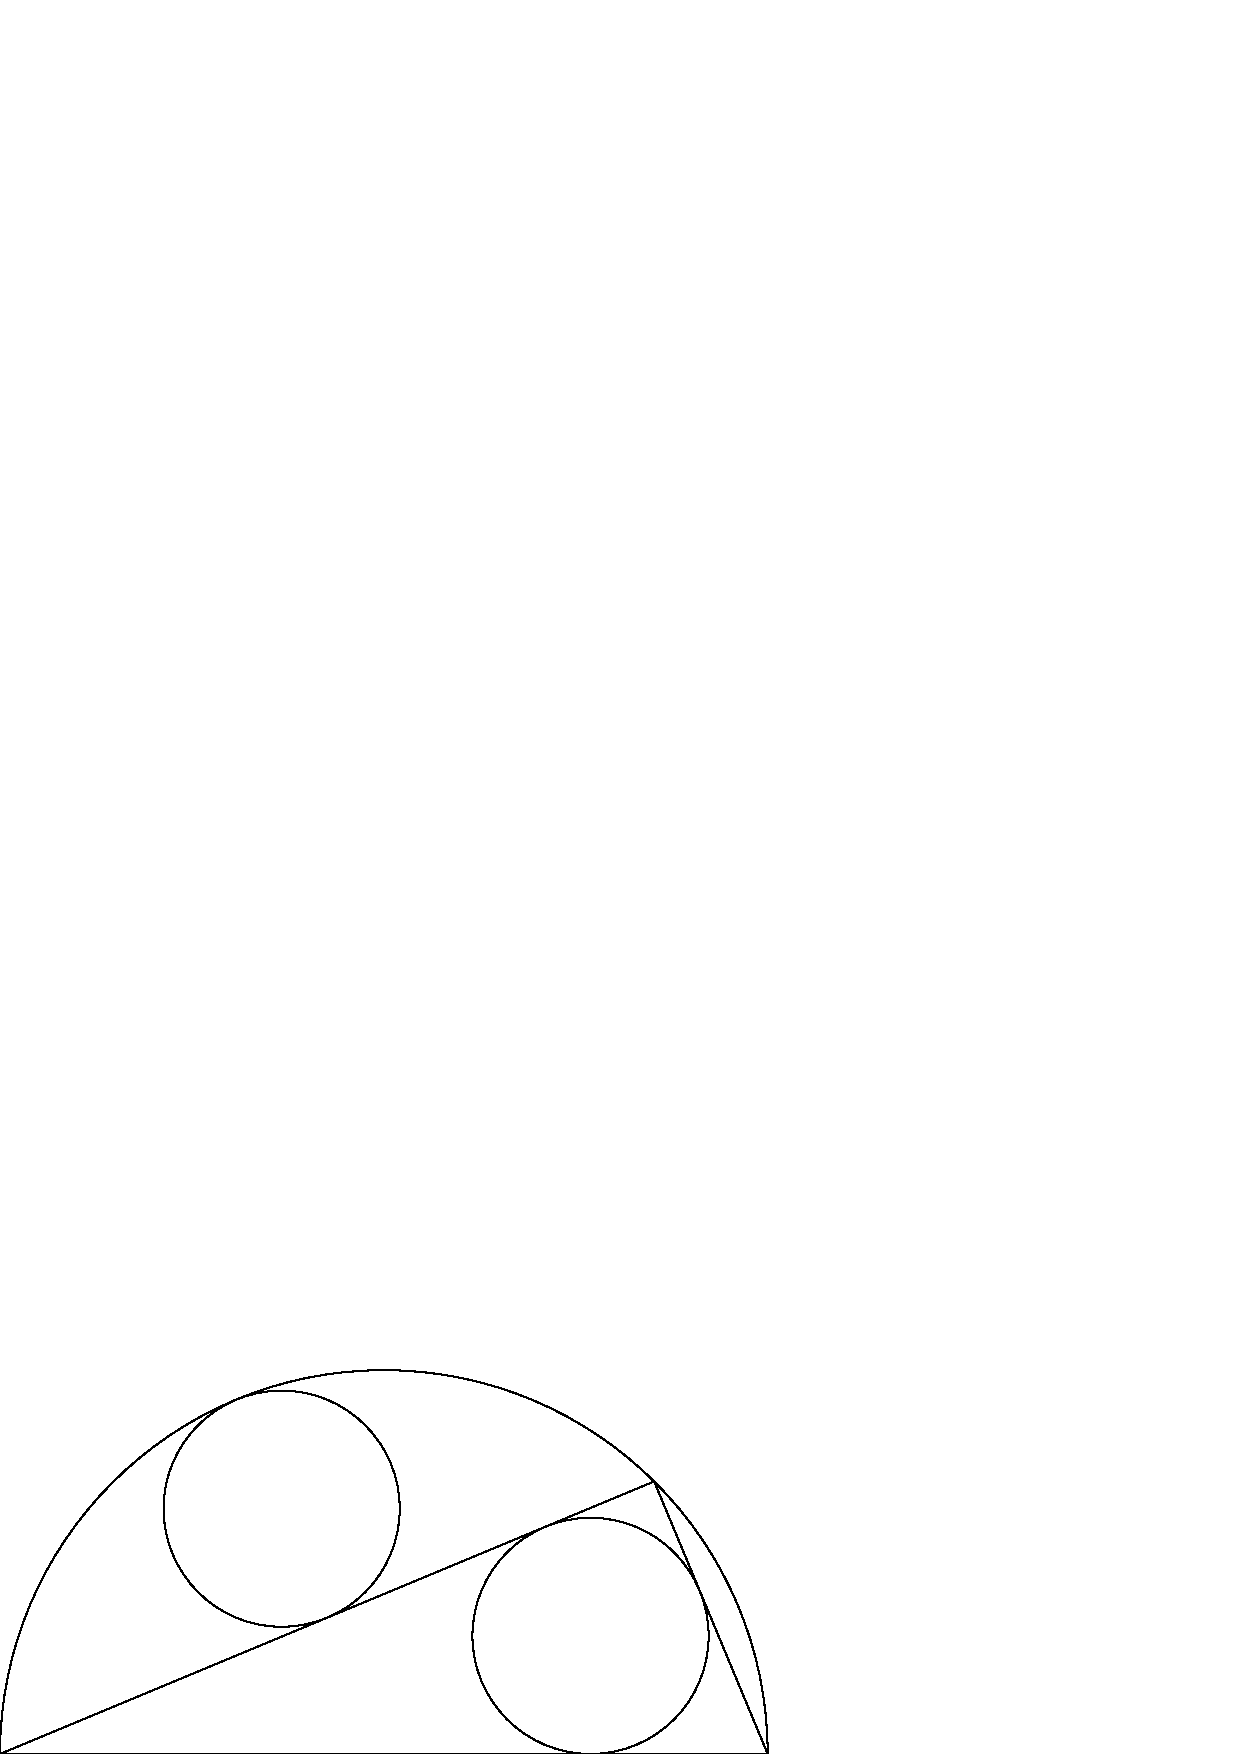
\includegraphics[height=8cm]{q1_0.pdf}
\end{center}


\section*{解答}

点や線を次の図のように定義する。

\begin{center}
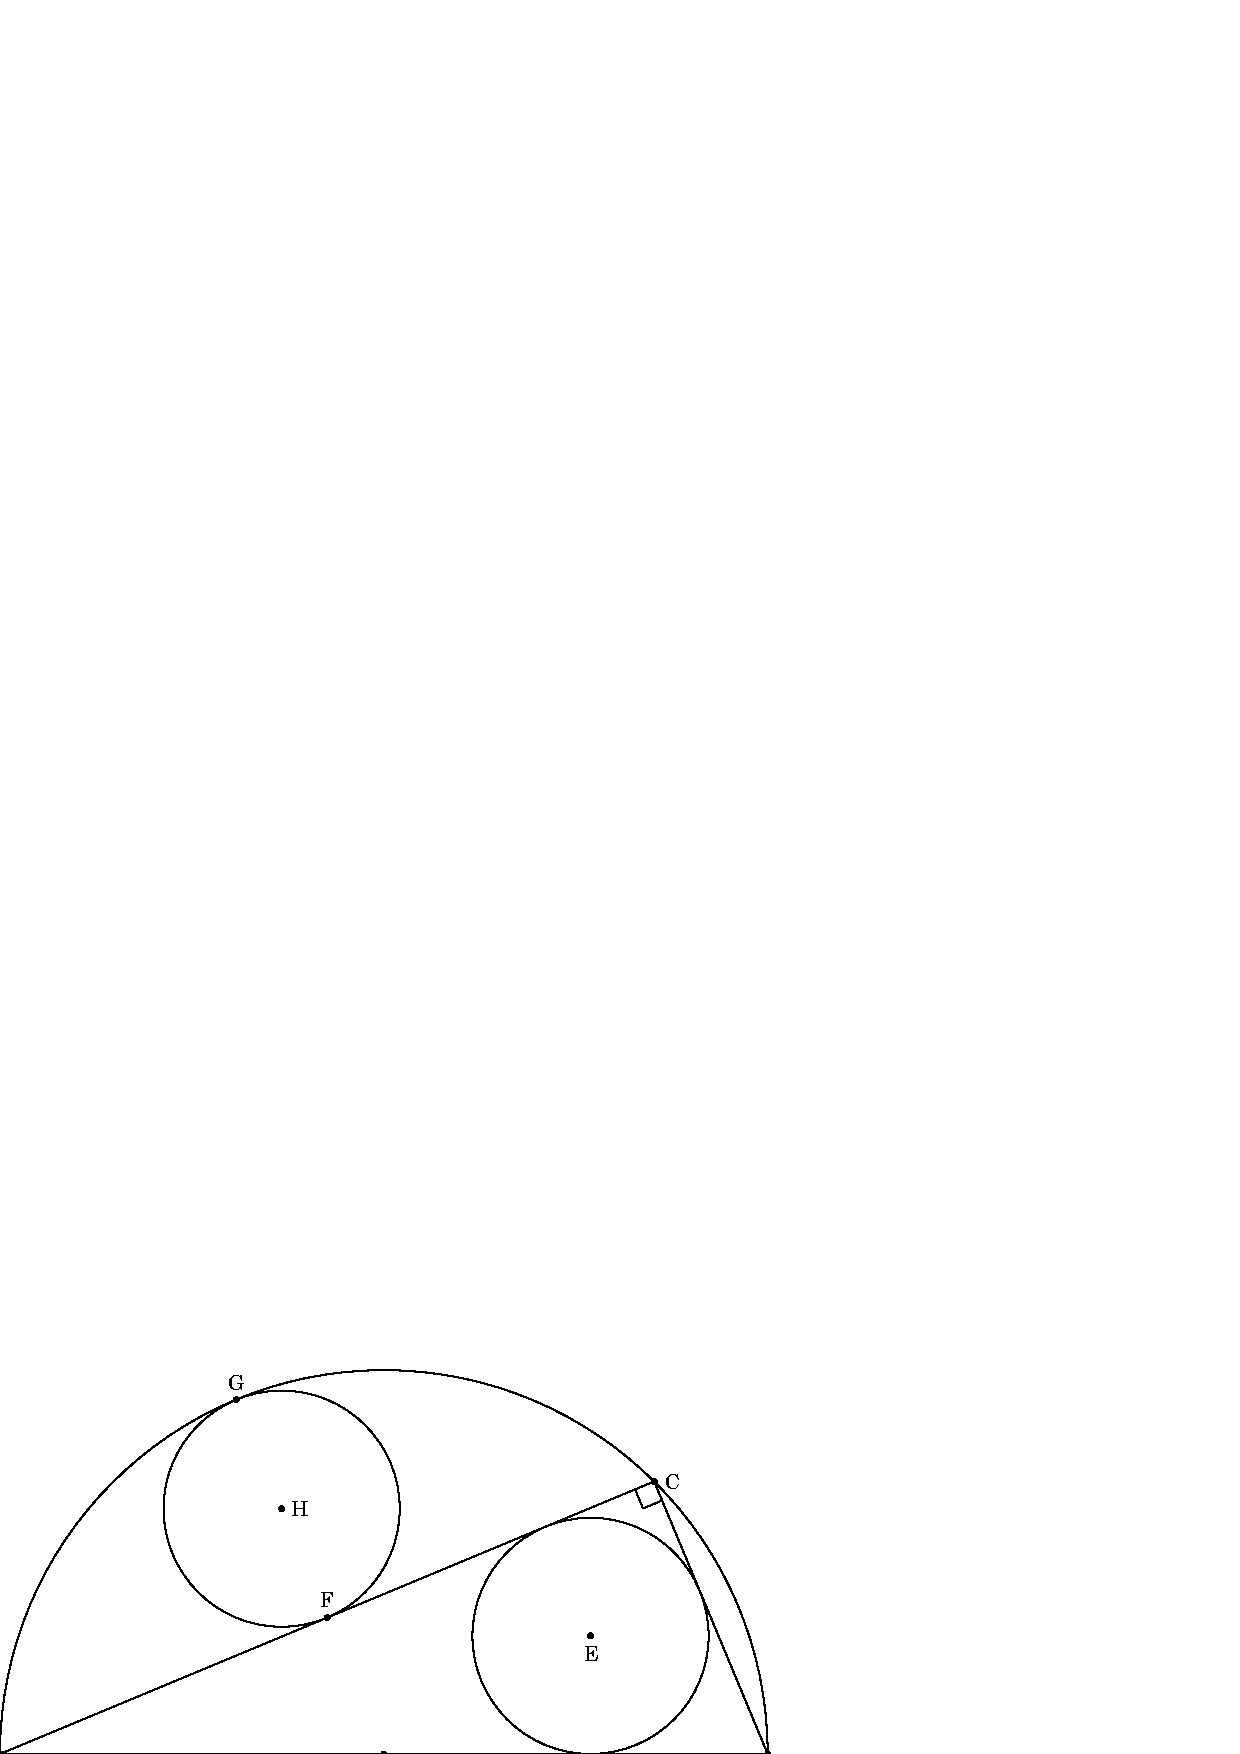
\includegraphics[height=8cm]{q1_1.pdf}
\end{center}

直線$AB$、直線 $BC$ 、直線 $CA$ はそれぞれEを中心とする小円の接線。
その接点をそれぞれ $I$、$J$、$K$ とする。

さらに、小円の半径を1、外接円の半径をR、${\angle}CAB=\theta^{\circ}$ とする。

\begin{center}
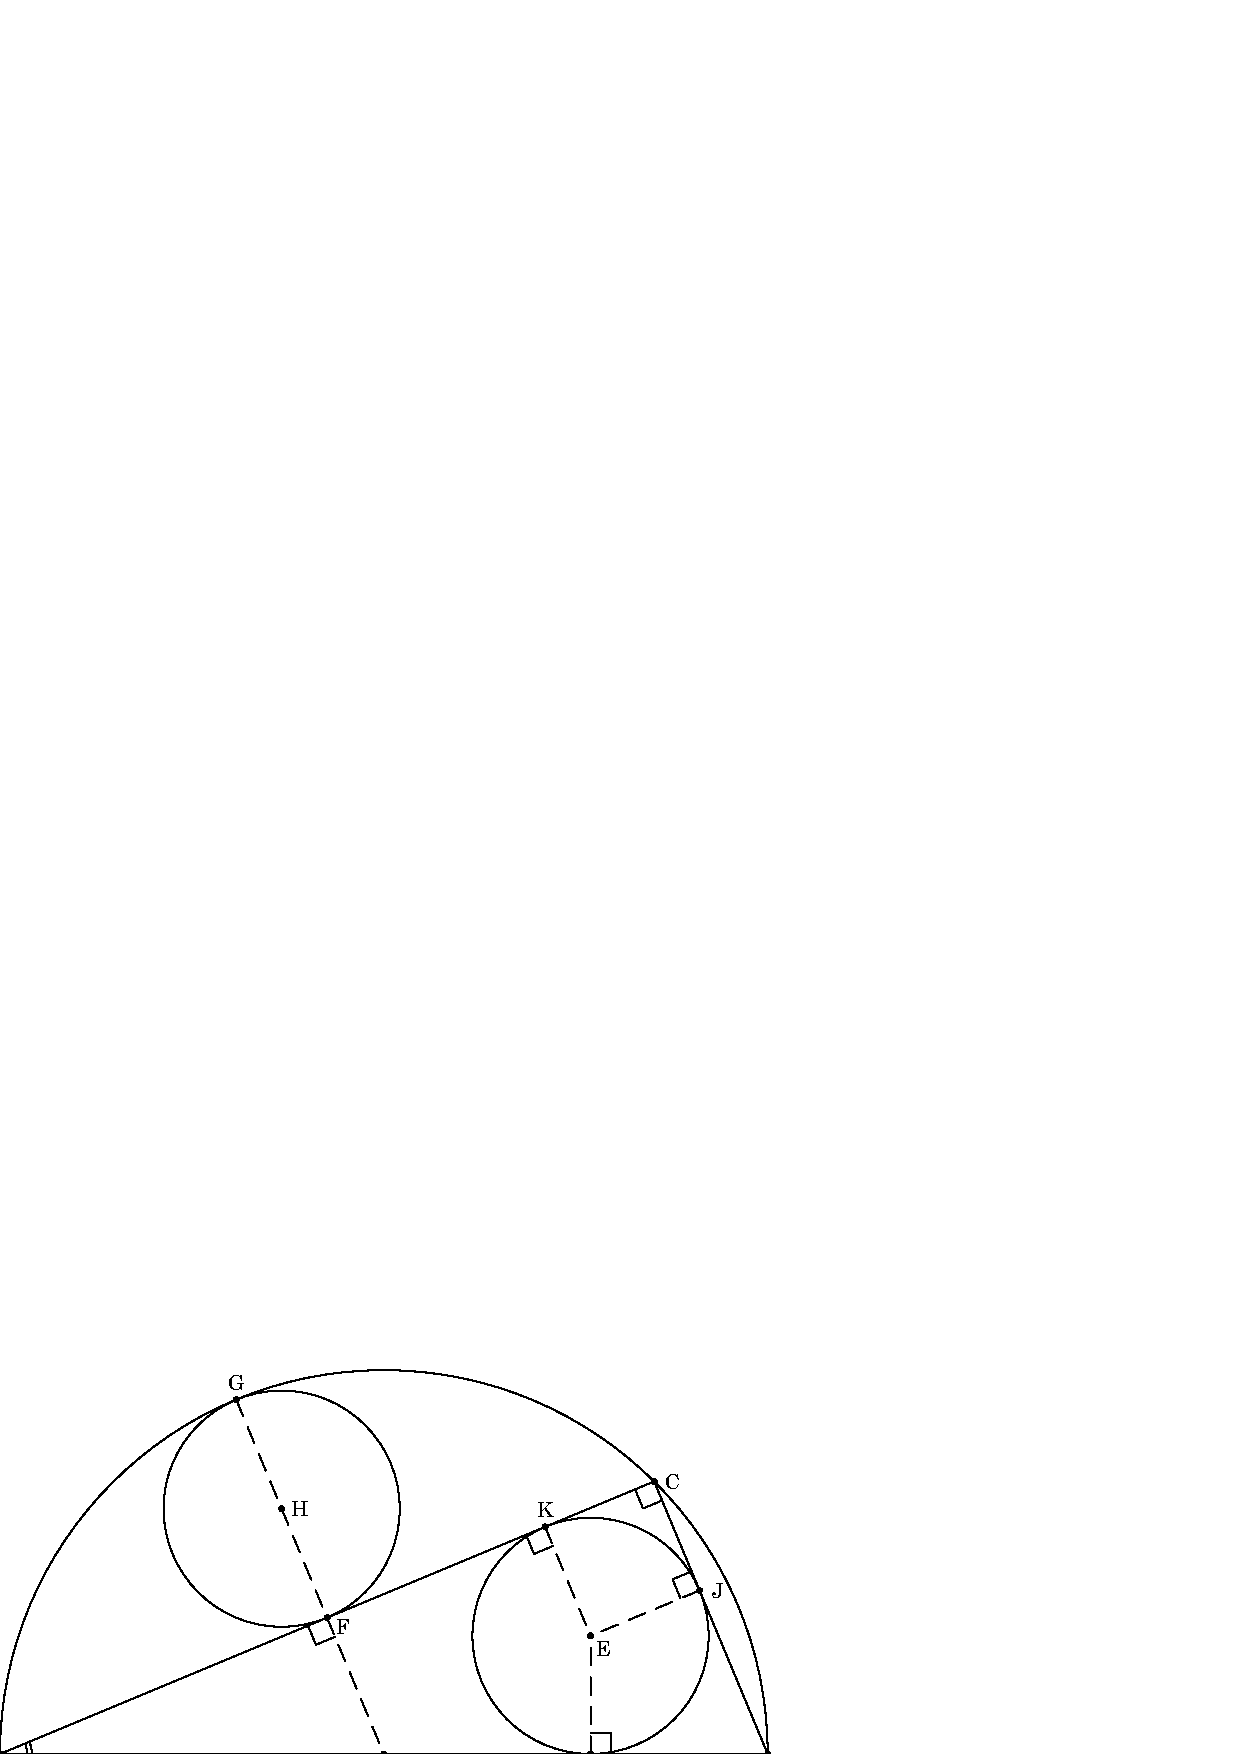
\includegraphics[height=8cm]{q1_2.pdf}
\end{center}

\newpage

まず、$AB$ を調べる。

$AB$ は外接円の直径のため、
\begin{gather}
 AB = 2R  \label{eq:ab1}
\end{gather}

また、
\begin{gather}
 AB = AI + IB  \label{eq:ab21}
\end{gather}

$AI$ と $AK$ はどちらも点 $A$ を通り、点 $E$ を中心とする小円の接線のため、
\begin{gather}
 AI = AK \label{eq:ai1}
\end{gather}

ここで、
\begin{gather}
 AC = AK + KC \notag \\
 AK = AC - KC \label{eq:ak1}
\end{gather}

三角形 $ABC$ において ${\angle}BCA = 90^{\circ}、{\angle}CAB = {\theta}^{\circ}$より、
\begin{gather}
 AC = AB{\cos}{\theta} \label{eq:ac11}
\end{gather}

\ref{eq:ab1}、\ref{eq:ac11} より、
\begin{gather}
 AC = 2R{\cos}{\theta} \label{eq:ac1}
\end{gather}

$KC$ と$EJ$ は正方形 $EJCK$ の2辺のため、
\begin{gather}
 KC = EJ \label{eq:kc1}
\end{gather}

$EJ$は小円の半径のため、
\begin{gather}
  EJ = 1 \label{eq:ej}
\end{gather}

\ref{eq:kc1}、\ref{eq:ej} より、
\begin{gather}
 KC = 1 \label{eq:kc}
\end{gather}

\ref{eq:ak1}、\ref{eq:ac1}、\ref{eq:kc} より、
\begin{gather}
 AK = 2R{\cos}{\theta} - 1 \label{eq:ak}
\end{gather}

\ref{eq:ai1}、\ref{eq:ak} より、
\begin{gather}
 AI = 2R{\cos}{\theta} - 1 \label{eq:ai}
\end{gather}

また、$IB$ と $BJ$ はどちらも点 $B$ を通り、点 $E$ を中心とする小円の接線のため、
\begin{gather}
 IB = BJ \label{eq:ib11}
\end{gather}

ここで、
\begin{gather}
 BC = BJ + JC \notag \\
 BJ = BC - JC \label{eq:bj1}
\end{gather}

三角形 $ABC$ において ${\angle}BCA = 90^{\circ}、{\angle}CAB = {\theta}^{\circ}$より、
\begin{gather}
 BC = AB{\sin}{\theta} \label{eq:bc11}
\end{gather}

\ref{eq:ab1}、\ref{eq:bc11} より、
\begin{gather}
 BC = 2R{\sin}{\theta} \label{eq:bc1}
\end{gather}

$JC$ と$EJ$ は正方形 $EJCK$ の2辺のため、
\begin{gather}
 JC = EJ \label{eq:jc1}
\end{gather}

\ref{eq:ej}、\ref{eq:jc1} より、
\begin{gather}
 JC = 1 \label{eq:jc}
\end{gather}

\ref{eq:bj1}、\ref{eq:bc1}、\ref{eq:jc} より、
\begin{gather}
 BJ = 2R{\sin}{\theta} - 1 \label{eq:bj}
\end{gather}

\ref{eq:ib11}、\ref{eq:bj} より、
\begin{gather}
 IB = 2R{\sin}{\theta} - 1 \label{eq:ib}
\end{gather}

\ref{eq:ab21}、\ref{eq:ai}、\ref{eq:ib}より、
\begin{gather}
 AB = 2R{\cos}{\theta} -1 + 2R{\sin}{\theta} -1 \notag \\
 AB = 2R{\sin}{\theta} + 2R{\cos}{\theta} - 2 \label{eq:ab2}
\end{gather}

\ref{eq:ab1}、\ref{eq:ab2} より、
\begin{gather}
 2R = 2R{\sin}{\theta} + 2R{\cos}{\theta} - 2 \notag \\
 R({\sin}{\theta} + {\cos}{\theta} - 1) = 1 \label{eq:ab}
\end{gather}

次に、$DG$ を調べる。

$DG$ は外接円の半径のため、
\begin{gather}
 DG = R \label{eq:dg1}
\end{gather}

一方、
\begin{gather}
 DG = DF + FG \label{eq:dg21}
\end{gather}

三角形ADFにおいて ${\angle}AFD=90^{\circ}$、${\angle}DAF={\theta}^{\circ}$ より、
\begin{gather}
 DF = AD{\sin}{\theta} \label{eq:df1}
\end{gather}

$AD$ は外接円の半径のため、
\begin{gather}
 AD = R \label{eq:ad}
\end{gather}

\ref{eq:df1}、\ref{eq:ad} より、
\begin{gather}
 DF = R{\sin}{\theta} \label{eq:df}
\end{gather}

FGはEを中心とする小円の直径のため、

\begin{gather}
 FG = 1 \times 2 \notag \\
 FG = 2 \label{eq:fg}
\end{gather}

\ref{eq:dg21}、\ref{eq:df}、\ref{eq:fg}より、

\begin{gather}
 DG = R{\sin}{\theta} + 2 \label{eq:dg2}
\end{gather}

\ref{eq:dg1}、\ref{eq:dg2}より、

\begin{gather}
 R = R{\sin}{\theta} + 2 \notag \\
 R = \frac{2}{1 - {\sin}{\theta}} \label{eq:dg}
\end{gather}

\ref{eq:ab}、\ref{eq:dg}より、

\begin{gather}
 \left\{
 \begin{array}{l}
  R({\sin}{\theta} + {\cos}{\theta} - 1) = 1 \\
  R = \dfrac{2}{1 - {\sin}{\theta}}
 \end{array}
 \right.
\end{gather}

\begin{gather*}
 \frac{2({\sin}{\theta} + {\cos}{\theta} - 1)}{1 - {\sin}{\theta}} = 1 \\
 2{\sin}{\theta} + 2{\cos}{\theta} -2 = 1 - {\sin}{\theta} \\
 {\cos}{\theta} = \frac{3}{2}(1 - {\sin}{\theta})
\end{gather*}

${\sin}^2{\theta} + {\cos}^2{\theta} = 1$より、
\begin{gather*}
 {\sin}^2{\theta} + [\frac{3}{2}(1 - {\sin}{\theta})]^2 = 1 \\
 13{\sin}^2{\theta} - 18{\sin}{\theta} + 5 = 0 \\
 {\sin}{\theta} = \frac{5}{13}, 1
\end{gather*}

${\theta}$は直角三角形の一角の角度で $0^{\circ} < {\theta}^{\circ} < 90^{\circ}$ のため、$0 < {\sin}{\theta} < 1$。よって、

\begin{gather}
 {\sin}{\theta} = \frac{5}{13}     \label{eq:sintheta}
\end{gather}

\ref{eq:dg}、\ref{eq:sintheta}より、

\begin{gather}
 R = \frac{2}{1 - \frac{5}{13}} \notag \\
 \therefore R = \frac{13}{4}
\end{gather}

そのため、小円の半径と外接円の半径の比は、$4:13$
\end{document}
